\section{Object Reconstruction}
\label{sec:reco}

This analysis selects events in which each top quark in a $t\bar{t}$ pair has decayed to a pair of quarks and a b jet that are merged into a single jet. Since the two quarks and b jet are all captured in a single boosted jet for each top quark, the jets in the event contain identifiable substructure. We utilize the standard CMS particle flow-based reconstruction of objects with the legacy Run 2 processing for data and MC. This analysis only uses jets, and hence does not select leptons or missing transverse momentum. The jet reconstruction and identification is discussed in this section.


\subsection{Jet Reconstruction}
\label{sec:jetreco}

We employ two jet collections clustered with the anti-$k_{\mathrm{T}}$ (AK) algorithm~\cite{antikt} with $R=0.4$ and $R=0.8$, reconstructed with the {\tt FASTJET} package~\cite{fastjet} referred to as ``AK4'' and ``AK8'' jets respectively. In order to mitigate the effects of pileup, "Charged Hadron Subtraction" is applied to the AK4 jets and "Pile Up Per Particle Identification'' (PUPPI) algorithm~\cite{puppi} is applied to the AK8 jets. The AK4 jet collection is used only for the construction of the $H_T$ variable, which is used to ensure the trigger efficiency is above 95\%. The rest of the analysis uses the AK8 jet collection with PUPPI. We require at least 2 top tagged AK8 jets. The jets are scaled by the Jet Energy Correction (JEC) factor~\cite{CMS:JEC} at the L1FastJet, L2Relative, L3Absolute levels. In data, an additional L2L3residual correction is applied to the jets. Since in our analysis we use both AK4 jets and AK8 jets, the corrections are applied to the AK4 and AK8 jets separately. The versions of the corrections applied are described in Table~\ref{tab:jerc}.


\begin{table}[!h]
	\centering
	\begin{tabular}{|ccc|} \hline
		Year       &  Jet Energy Corrections  &  Jet Energy Resolution   \\ \hline
		2016    &  Summer19UL16APV\_V7     &  Summer20UL16APV\_JRV3      \\
		&  Summer19UL16\_V7        &  Summer20UL16\_JRV3      \\
		2017         &  Summer19UL17\_V5        &  Summer19UL17\_JRV2   \\
		2018         &  Summer19UL18\_V5        &  Summer19UL18\_JRV2   \\\hline
	\end{tabular}
	\caption{JEC and JER versions used for each year in this analysis.}
	\label{tab:jerc}
\end{table}


\subsection{Top Quark Identification}

% I see deepAK8 but I don't see deepAK8 mass decorrelated , what it is ??? WE NEED A DISCUSSION ON THAT. 

In choosing the top tagger for this analysis, we compared ParticleNet, DeepAK8, HOTVR \cite{HOTVR}, and the CMS Top Tagger v2 (CMSv2). CMSv2 is a cut-based tagger based on an nsubjettiness cut combined with a soft drop mass window cut, $\tau_{32} < 0.65$ and $105 GeV < m_{SD} < 210 GeV$. The DeepAK8 tagger was determined to be the optimal tagger for this analysis, as it has better performance than the previously used CMSv2 tagger and is also used in the semileptonic channel of this $t\bar{t}$ analysis. Since this analysis relies heavily on a well-understood background estimate utilizing extrapolations of sidebands, we utilize the version of the tagger that has used mass decorrelation. This is a critical feature for the background estimate. 

The DeepAK8 tagger is a deep neural network (DNN) that classifies the signal of a heavy resonance decay from QCD background. The DNN takes the kinematic information of PF candidates as input variables, as well as secondary vertex and charged particle track information. The base version of DeepAK8 is correlated with the jet mass, which results in mass sculpting of background events. For our analysis we need a tagger that is mass decorrelated, as the background estimate is dependent on the jet mass. DeepAK8 has a mass decorrelated version (DeepAK8MD) that uses adversarial training to regulate the behavior of the tagger. We use the TvsQCD classification of the DeepAK8MD tagger, which distinguishes jets from top quark decays from other hadronic jets.  



% This is done for the deepAK8 mass decorrelated. The plots with the shape difference in different tagger intervals indicates a corrleation at low tagger score. Not sure if this discussion should be here. I think it should be in the background estimation study.

%Figures \ref{fig:2Ddeepak8} - \ref{fig:deepak8Windows2} shows DeepAK8's relation to the jet mass and $p_T$, demonstrating the usefulness of the tagger to pick out tops from QCD background.  Placing a cut close to a discriminator value of 1 gives a tighter selection on top events.  Values within a range of $[0.0,\ 0.2)$ gives distributions that are not always consistent with the other ranges, which can be seen in Figures \ref{fig:deepak8Windows1} and \ref{fig:deepak8Windows2}.  

While ParticleNet has better top tagging efficiency, it does not have a mass decorrelated version, which is necessary for the background estimation.
%
%\begin{figure}[!htbp]
%  \begin{center}
%    \includegraphics[width=0.50\textwidth=0.2]{Plots/tagger/ROC_tagger.png}
%    \caption{ROC curves for DeepAK8, HOTVR, and CMS top tagger v2 with comparisons to the DeepAK8 2016 working points.}
%    \label{fig:roc_tagger}
%  \end{center}
%\end{figure}
%


%\subsection{b Tagger}
%
%Our b-tagger is another DNN, DeepCSV, that was trained to discriminate between jets, both AK4 and subjets, that originate from b quark decay vs lighter quarks. For b-tagging, we check the subjets of both AK8 jets.  Therefore, we place a further requirement on the pair of AK8 jets to have 2 subjets (i.e. a successful completion of the soft drop algorithm).  An AK8 jet is considered to be b-tagged if at least one of its subjets pass the tagger cut \cite{BTVwiki}:
%
%\begin{itemize}
%\item {\bf 2016APV:} {\tt DeepCSV} $>\ 0.6001$
%\item {\bf 2016:} {\tt DeepCSV} $>\ 0.5847$
%\item {\bf 2017:} {\tt DeepCSV} $>\ 0.4506$
%\item {\bf 2018:} {\tt DeepCSV} $>\ 0.4506$  
%\end{itemize}
%
%\clearpage

\section{Event Selection Summary}

% You need the distribution of the reconstructed signal observables such as delta phi , HT, you can also show the reconstructed mass of the Heavy particles i.e  $Z^{'}$ $m_{TTbar}$}

We apply a preselection on the $p_T$, rapidity ($y$), $|\Delta \phi|$ between the two ttbar candidate AK8 jets. We use rapidity instead of pseudorapidity because the AK8 jets produced by top quarks are massive. The distribution of $H_T$ before the preselection and the distribution of $p_T$ of the leading AK8 jet of SM TTBar and 2 TeV RSGluon datasets are shown in Figures~\ref{fig:kin2016}-~\ref{fig:kin2018}.


\begin{figure}[htp]
	\begin{center}
		\includegraphics[width=0.45\textwidth]{Plots/kinematics/2016all/jetpt_inclusive.pdf}
		\includegraphics[width=0.45\textwidth]{Plots/kinematics/2016all/jetphi_inclusive.pdf}
		\includegraphics[width=0.45\textwidth]{Plots/kinematics/2016all/jeteta_inclusive.pdf}
		\includegraphics[width=0.45\textwidth]{Plots/kinematics/2016all/jety_inclusive.pdf}
		
		\caption{$p_T$, $\phi$, and  $\eta$ of the leading AK8 jet for the 2016 SM TTbar and 2 TeV RSGluon datasets.}
		\label{fig:kin2016}
	\end{center}
\end{figure}

\begin{figure}[htp]
	\begin{center}
		\includegraphics[width=0.45\textwidth]{Plots/kinematics/2017/jetpt_inclusive.pdf}
		\includegraphics[width=0.45\textwidth]{Plots/kinematics/2017/jetphi_inclusive.pdf}
		\includegraphics[width=0.45\textwidth]{Plots/kinematics/2017/jeteta_inclusive.pdf}
		\includegraphics[width=0.45\textwidth]{Plots/kinematics/2017/jety_inclusive.pdf}
		
		\caption{$p_T$, $\phi$, and  $\eta$ of the leading AK8 jet for the 2017 SM TTbar and 2 TeV RSGluon datasets.}
		\label{fig:kin2017}
	\end{center}
\end{figure}

\begin{figure}[htp]
	\begin{center}
		\includegraphics[width=0.45\textwidth]{Plots/kinematics/2018/jetpt_inclusive.pdf}
		\includegraphics[width=0.45\textwidth]{Plots/kinematics/2018/jetphi_inclusive.pdf}
		\includegraphics[width=0.45\textwidth]{Plots/kinematics/2018/jeteta_inclusive.pdf}
		\includegraphics[width=0.45\textwidth]{Plots/kinematics/2018/jety_inclusive.pdf}
		
		\caption{$p_T$, $\phi$, and  $\eta$ of the leading AK8 jet for the 2018 SM TTbar and 2 TeV RSGluon datasets.}
		\label{fig:kin2018}
	\end{center}
\end{figure}



\subsection{Kinematic Selection}


The following event selection is applied: 


\begin{itemize}
\item $\ge 2$ AK8 jets with $\pt > 400$ GeV, $|y| < 2.4$, $|\eta| < 2.4$, and loose jet ID (jetID $>$ 0 \cite{jetid})
\item $|\Delta \phi| > 2.1$ between two leading AK8 jets. 
\item $H_T > 1400$ GeV (calculated with AK4 jets) with ${\mathrm{p}}^{\mathrm{AK4}}_{\mathrm{T}}$ $>$ 30 and $|\eta^{\mathrm{AK4}}|$ $<$ 3.0; $H_T\ =\ \sum_i^{\mathrm{AK4\ Jets}}{p_{Ti}}$ (the cut value was determined by the trigger efficiency, discussed in Section~\ref{sec:trigeff})

\end{itemize}


\subsection{Trigger Selection}
\label{sec:trigeff}


The data were collected with a trigger based on the total scalar sum of transverse momenta of PF jets in the event (PFHT). Substructure based triggers such as AK8PFTH800\_TrimMass50 and similar are not used in this analysis because they bias the background estimate.


\subsection{Signal Selection}
\label{sec:signal}

The signal region is then defined by the two AK8 jets passing the 0.1\% Working Point (WP) for the mass decorrelated DeepAK8 top tagger (DeepAK8MD)~\cite{DeepAK8TopTagwiki}. The 0.1\% WP corresponds to a mistag rate of 0.1\%, and the discriminator values for each year are shown in Table~\ref{tab:deepak8}. There is also a requirement for the signal region of $105 < m_t < 210$ GeV, where $m_t$ is the softdrop mass of the leading jet.

\begin{table}[h!]
	\centering
	\begin{tabular}{|| c c  ||} 
		\hline
		Year & Discriminator Cut \\ 
		\hline\hline
		2016 & 0.889  \\ 
		2017 & 0.863  \\ 
		2018 & 0.920  \\ 
		\hline
	\end{tabular}
	\caption{Discriminator values for the 0.1\% WP for the DeepAK8MD tagger.}
	\label{tab:deepak8}
\end{table}


\subsection{Event Categorization}
\label{sec:selection}


% Add discussion on delta Y as well as support figures.


In the previous analysis, the events are divided into regions based on top tags, b-tags, and a rapidity cut for better signal purity. However, the DeepAK8MD tagger is correlated with the b-tagger, so we only split the analysis into the rapidity regions, a central region ($\Delta y < 1.0$) and a forward region ($\Delta y > 1.0$). The distribution of the $\Delta Y$ between the two leading AK8 jets is shown in Figure~\ref{fig:jety}.


\begin{figure}[htp]
	\begin{center}
		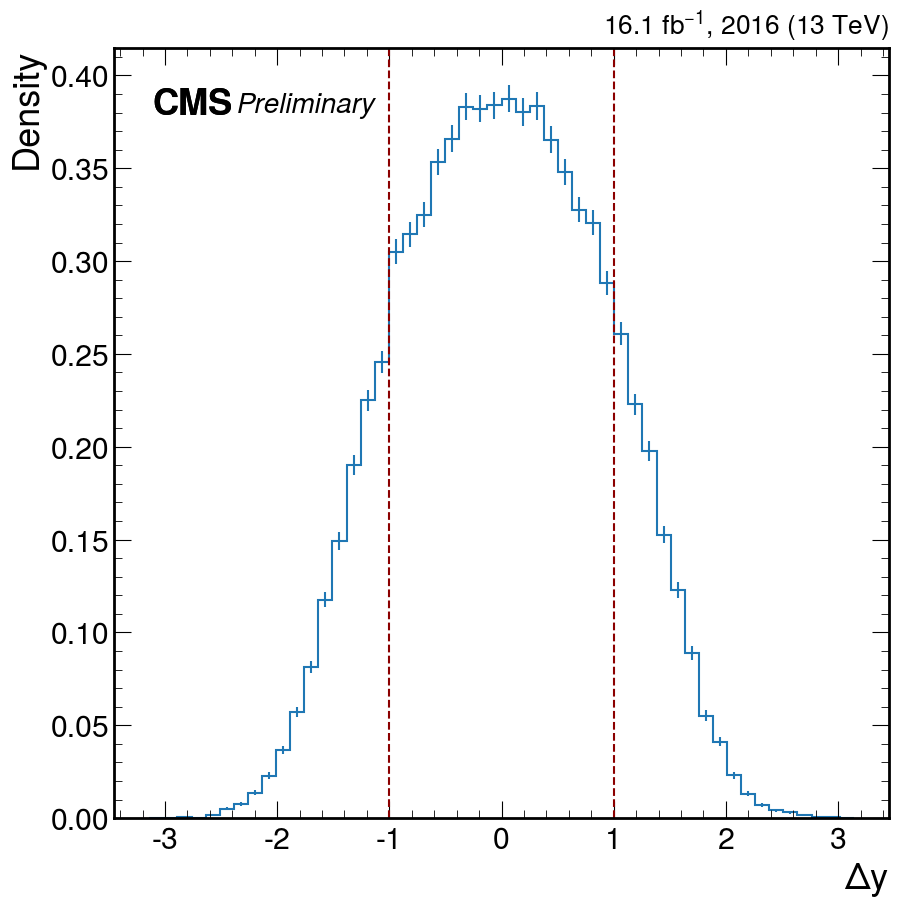
\includegraphics[width=0.3\textwidth]{Plots/kinematics/delta_rapidity.png}
		\caption{Difference in rapidity of the two AK8 jets in the $t\bar{t}$ candidate for the 2016APV datasets for the 2 TeV RSGluon.}
		\label{fig:jety}
	\end{center}
\end{figure}

\subsection{MET Filters}

We also apply the following MET filters for all UL Run II Data and MC as recommended by the JetMET POG:

\begin{itemize}
	\item {primary vertex filter}
	\item {beam halo filter}
	\item {HBHE noise filter}
	\item {HBHEiso noise filter}
	\item {ECAL TP filter}
	\item {ECAL Bad Calibration Filter}
	\item {Bad PF Muon Filter}
	\item {Bad PF Muon Dz Filter}
	\item {ee badSC noise filter}
	\item {HF noisy hits filter}
	
\end{itemize}


\subsection{Summary}


The event selection cuts and corresponding event counts in data for all years are listed in Table~\ref{tab:cutflow}.

\begin{table}
	\begin{center}
		\rowcolors{2}{gray!15}{white}
		\begin{tabular}{|p{4cm}||p{2cm}||p{2cm}||p{2cm}||p{2cm}|   } \hline 
			\textbf{Cut} & \textbf{2016 Events} & \textbf{2017 Events} & \textbf{2018 Events} & \textbf{Total Events} \\ \hline
			All Events                                 &  625,441,538  &  409,943,376 &  676,743,923  &  1,712,128,837 \\
			Trigger                                     &  77,080,857  &  37,942,480 &  44,303,284  &  159,326,621 \\
			$HT > 1400$                                 &  6,860,501  &  8,082,202 &  10,212,075  &  25,154,778 \\
			METFilter                                   &  6,800,777  &  8,024,727 &  10,159,014  &  24,984,518 \\
			AK8 JetId $>$ 1               &  6,800,639  &  8,024,617 &  10,158,742  &  24,983,998 \\
			AK8 $p_T > 400$ GeV, $|y| < 2.4$    &  6,766,299  &  7,993,862 &  10,108,968  &  24,869,129 \\
			$>=2$ AK8 Jets                               &  6,228,125  &  7,436,018 &  9,276,096  &  22,940,239 \\
			$|\Delta\varphi| > 2.1$                     &  6,154,529  &  7,344,374 &  9,170,042  &  22,668,945 \\
			\hline
		\end{tabular}
		\caption{Cutflow for JetHT events for 2016, 2017 and 2018 datasets.}
		\label{tab:cutflow}
	\end{center}
\end{table}





\subsection{HEM 15/16 Correction}

For the 2018 datasets, we take into account failures in the HCAL Endcap Minus (HEM) 15 and 16. During the last certified run of 2018B and all of 2018C and 2018D, the power supply in two HCAL modules died, impacting the jet energy measurement in this region. We apply a veto for any events with jets with $-1.57 < |\phi| < -0.87$ and $-2.5 < |\eta| < -1.3$, and jets with $-1.57 < |\phi| < -0.87$ and $-3.0< |\eta| < 2.5$. The HEM veto cuts out less than 2\% of the 2018 data.






%\section{Corrections}


%\subsection{Jet Energy Scale and Resolution}
%
%The jets are scaled by the Jet Energy Correction (JEC) factor~\cite{CMS:JEC} at the L1FastJet, L2Relative, L3Absolute levels. In data, an additional L2L3residual correction is applied to the jets. Since in our analysis we use both AK4 jets and AK8 jets, the corrections are applied to the AK4 and AK8 jets separately. The versions of the corrections applied are described in Table~\ref{tab:jerc}.
%
%
%\begin{table}[!h]
%  \centering
%  \begin{tabular}{|ccc|} \hline
%  Year       &  Jet Energy Corrections  &  Jet Energy Resolution   \\ \hline
%  2016    &  Summer19UL16APV\_V7     &  Summer20UL16APV\_JRV3      \\
%   	    &  Summer19UL16\_V7        &  Summer20UL16\_JRV3      \\
%  2017         &  Summer19UL17\_V5        &  Summer19UL17\_JRV2   \\
%  2018         &  Summer19UL18\_V5        &  Summer19UL18\_JRV2   \\\hline
%  \end{tabular}
% \caption{JEC and JER versions used for each year in this analysis.}
%\label{tab:jerc}}
%\end{table}


\subsection{Top Tagging Scale Factor}

The top tagging scale factor is implemented to account for differences in the efficiency of the top tagging in simulation and data. The scale factor is calculated as an unconstrained nuisance parameter that is extracted from the fit.


%\section{Data quality mitigation issues}

\subsection{Pileup}

The samples are generated with a different pileup distribution than the data, so they are reweighted to have a matching distribution for the number of interactions. This is done by reweighting the generated number of PU vertices in the MC to match the data, using the jsonPOG files \cite{jsonPOG}. This package is also used to propagate the uncertainty in the total inelastic cross section and is accounted for in the analysis. 


\subsection{L1 Prefiring Correction}

We take into account the effect of a timing shift in the ECAL subdetector that resulted in the Level-1 Trigger incorrectly assigning trigger flags to the previous bunch crossing. The prefiring weights depend on $p_T$ and $\eta$ and are the product of the non-firing probability of all objects in the event. We apply these corrected weights to the events of the simulated samples as suggested by ~\cite{L1prefiring}. 





